\section{SMARTHEP as a European Training Network}
\label{network}
As a European Training Network (ETN), the primary aim of the network is in training ESRs, whilst deepening synergies between HEP and industry. The network takes a novel approach to building such synergies, structuring each ESR position (a 3 year period of doctoral study) around academic and industrial secondments. To achieve this, the network is formed of a series of partnerships between universities, research institutes and organisations in industry, as listed in Table~\ref{partners}.\par

\begin{table}[h!]
    \centering
    \small
    \begin{tabular}{p{2.5cm}p{9.5cm}}
    \hline
    Category & Partners \\\hline
    Universities & Lund University, Sorbonne University (LPNHE \& LIP), Technische Universit\"at Dortmund, University of Bologna, University of Geneva, University of Heidelberg, University of Helsinki, University of Manchester, Universidade Santiago de Compostela (IGFAE), Vrije Universiteit Amsterdam \\\hline
    Research institutes & CERN, CNRS, NIKHEF  \\\hline
    Industry partners & IBM France, Lightbox, Point 6, Uni.versity of Manchester Institute for Data Science and AI, Verizon Connect, Ximantis\\\hline
    \end{tabular}
    \caption{The 18 organisations which form the SMARTHEP network.}
    \label{partners}       
\end{table}

The network is formally structured as 7 Work Packages (WPs), laid out in Figure~\ref{network-diagram}. WP1 ``Management'', covers the management of the network by the Project Manager/Project Coordinator/Executive Board. WP2 ``Training'', sets out training and development of participants, by both network partners and external training providers. WP3 ``Machine learning \& advanced data analysis'', develops machine learning (ML) techniques for use in real-time environments. WP4 ``Hybrid architectures'' focuses upon the deployment of non-CPU computing architectures in acceleration of data processing. WP5 ``Decision-making in research and industry'', applies WP3 and WP4 to develop RTA-based decision-making technologies. WP6 ``Monitoring and discoveries'', also applies WP3 and WP4 to RTA approaches in data analysis. WP7 ``Dissemination and communication of results'', publishes and propagates the results produced in WP6 and WP7.\par
\begin{figure*}[h!]
    \centering
    % Use the relevant command for your figure-insertion program
    % to insert the figure file. See example above.
    % If not, use
    %\vspace*{5cm}       % Give the correct figure height in cm
    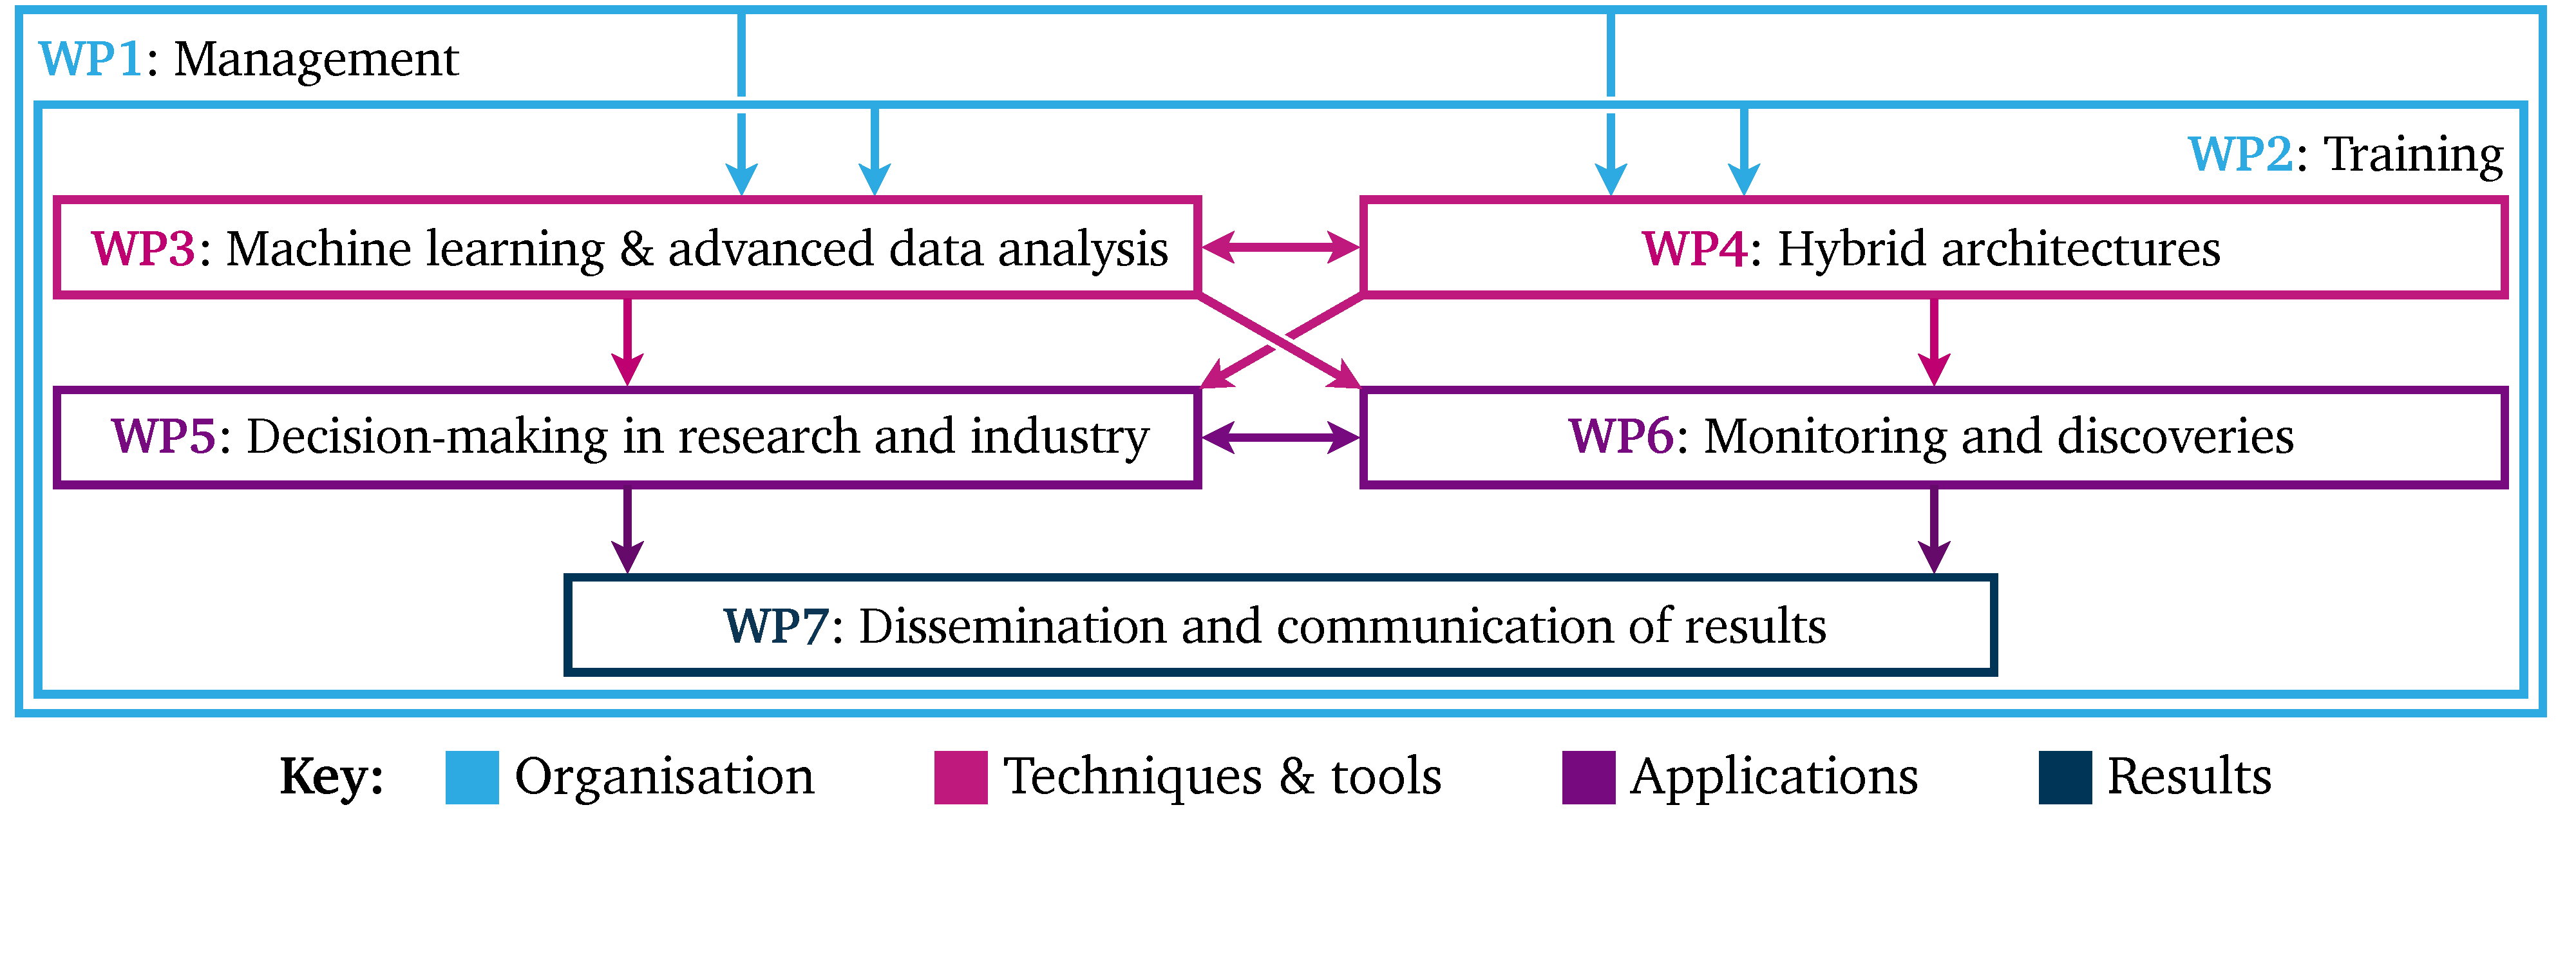
\includegraphics[width=0.9\linewidth]{/Users/jgooding/Documents/SMARTHEP/CHEP2023/CHEP2023/proceedings/figures/network-diagram.pdf}
    \caption{The structure of work packages within the SMARTHEP network. WP1 and WP2 define the organisation of the network; WP3 and WP4 introduce the techniques and tools of real-time analysis to the network; WP5 and WP6 use said techniques and tools to produce results for HEP and industry; WP7 makes these results available and promotes their wider use and adoption.}
    \label{network-diagram}       % Give a unique label
\end{figure*}

The network has a particular focus on physics at the Large Hadron Collider (LHC). Each ESR is thus affiliated to one of the four major experiments based at the LHC: ALICE, ATLAS, CMS and LHCb. The network duration coincides with Run 3 of the LHC (2022-2025), with many of the ESR projects framed in this context.\par

A unique feature of the network is the extensive cooperation between HEP and industry across all ESR positions.  RTA approaches have seen significant adoption in industry in recent years, with many organisations turning to RTA as a means to handle ``big data''.\par